\section{The meaning of Necessity}
\label{s:semantics}

In the introduction we spoke of \emph{Necessity Specifications}, e.g., $\onlyIf {A_1} {A_2} {A_3}$. 
% There are three, related, forms of necessity specifications, i.e. $\onlyIf {A_1} {A_2} {A_3}$,
% $\onlyIf {A_1} {A_2} {A_3}$, and 
% $\onlyThrough {A_1} {A_2} {A_3}$, $\onlyIf {A_1} {A_2} {A_3}$.
In this section we will define the semantics of such specifications.
In order to do that, we first define 
an underlying programming language \Loo, (Section \ref{sub:Loo}).
We then  define an assertion language, \SpecO,  which can talk about
 the contents of the state, as well about 
  of provenance and permission (Section \ref{sub:SpecO}).
Finally, we define necessity specifications in \Chainmail (Section \ref{s:holistic-guarantees}).



\subsection{\Loo}
\label{sub:Loo} 
\jm[TODO: mention the type system and the restriction on external method calls]{}
% We introduce a simple object-oriented language, \Loo, upon 
% which our specification language sits.
 \Loo is a small, simple, imperative,
class based, object oriented language. 
Given the simplicity of \Loo, we do not
define it here, \sd{instead,} we direct the reader to Appendix \ref{app:loo} for 
the full \sd{definitions}. % syntax and operational semantics.
\sd{Here we outline the definitions, and  introduce the concepts most relevant to the
treatment of the open world guarantees.}

A \Loo state $\sigma$ consists of a 
heap $\chi$, and a \jm[]{stack $\psi$, which is a sequence of frames $\phi$}.
A frame $\phi$ consists of
local variable map, and \sd{a continuation}, i.e. a sequence of statements to be executed.
 A statement may \sd{assign to variables}, create new objects and push them to the heap, 
perform field reads and writes on objects,  \sd{or}
 call methods on those objects. 

%Program 
\sd{Execution} is performed in the context of a module $M$,
which is a mapping
\sd{from} class names to class definitions. 
\sd{Execution has the format}  $M, \sigma \leadsto \sigma'$, has a small-step semantics, and is
unsurprising,  c.f. Appendix \ref{app:loo}.
\sd{The statements being executed are those in the continuation of the top frame.}
 % chopped, as generic 
 % There are several properties  of \Loo that are important to the central topic of this paper. 
 
As we said in section \ref{s:approach}, we are interested in guarantees which hold
when the external module is executing, and are not concerned if the internal module  temporarily
breaks them. Therefore, we are only interested in states where the
executing object (the \prg{this}) is an external object. 
For this, we define the  \emph{external state semantics}, of the form 
$\reduction{M_1}{M_2}{\sigma}{\sigma'}$, where $M_1$ is the external
module, and $M_2$ is the internal module, and where we
collapse all internal steps into one single step.

 
% SD removed, as disagreed with some of what is said below
% which allow us to 
%we define two forms of the operational semantics for \Loo, one in Fig. \ref{f:loo-semantics}
%that is unsurprising and details the execution of specific 
%statements in the language, and a second called \emph{external state semantics} 
%that models that open world, where the components of a program can
%have both known (\internalO) and unknown (\externalO) provenance.


\begin{definition}[External State Semantics]
\label{def:pair-reduce}
For  
% If we say "internal module", it is sounds as something makes the module be internal
  modules $M_1$,  $M_2$, and program states $\sigma$, $\sigma'$, 
we say that $\ \ \ \ \ \ \ \ \reduction{M_1}{M_2}{\sigma}{\sigma'}\ \ \ \ \ \ \ \ $ if and only if there exists a 
$n\in\mathbb{N}$, such that
\begin{itemize}
% SD changed because the old version was slightly wrong
\item
\sd{$\sigma$=$\sigma_1$, and  $\sigma'$=$\sigma_n$},
\item
$M_1 \circ M_2, \sigma_i \leadsto \sigma_{i+1}$  \ \ \ for all $i\in [0..n)$,
\item
$\class{\sigma}{\sigma.\prg{this}}, \class{\sigma'}{\sigma'.\prg{this}}\in M_2$,
\item
$\class{\sigma_i}{\sigma_i.\prg{this}} \in M_1$\ \ \ for all $i\in [1..n)$.
\end{itemize} 
%$M_1 \circ M_2, \sigma \leadsto \sigma_1 \leadsto \ldots \sigma_n \leadsto \sigma'$ and $\class{\sigma_i}{\sigma_i.\prg{this}} \in M_1$ for all $0 \leq i \leq n$
%
%$\class{\sigma}{\sigma.\prg{this}}\ \in\ M_2$ and
%\item
%$\class{\sigma'}{\sigma'.\prg{this}}\ \in\ M_2$ and 
%\end{itemize} 
%%and
%%\begin{itemize}
%%\item
%%$\exec{M_1\ \circ\ M_2}{\sigma}{\sigma'}$ or
%%\item
%$M_1 \circ M_2, \sigma \leadsto \sigma_1 \leadsto \ldots \sigma_n \leadsto \sigma'$ and $\class{\sigma_i}{\sigma_i.\prg{this}} \in M_1$ for all $0 \leq i \leq n$
%\end{itemize}
\end{definition}
In Definition \ref{def:pair-reduce}  % of external state semantics makes reference to a 
we  use  the function
$\class{\sigma}{x}$. This function looks up 
the class of   the object referred by variable $x$ in the heap of $\sigma$. 
  % for a specific variable in a specific program.
% SD not a variable, and no program.
We also use module linking, $M_1\circ M_2$. The operator $\circ$
 %  results in the union of two disjoint modules.
\sd{combines the two modules into one module in the obvious way, provided that their 
domains are disjoint.}
Full details in  Appendix \ref{app:loo}.
\begin{figure}[htb]
  \vspace*{-2.5mm}
  \begin{center}
   \begin{minipage}{0.80\textwidth}
     \begin{center}
       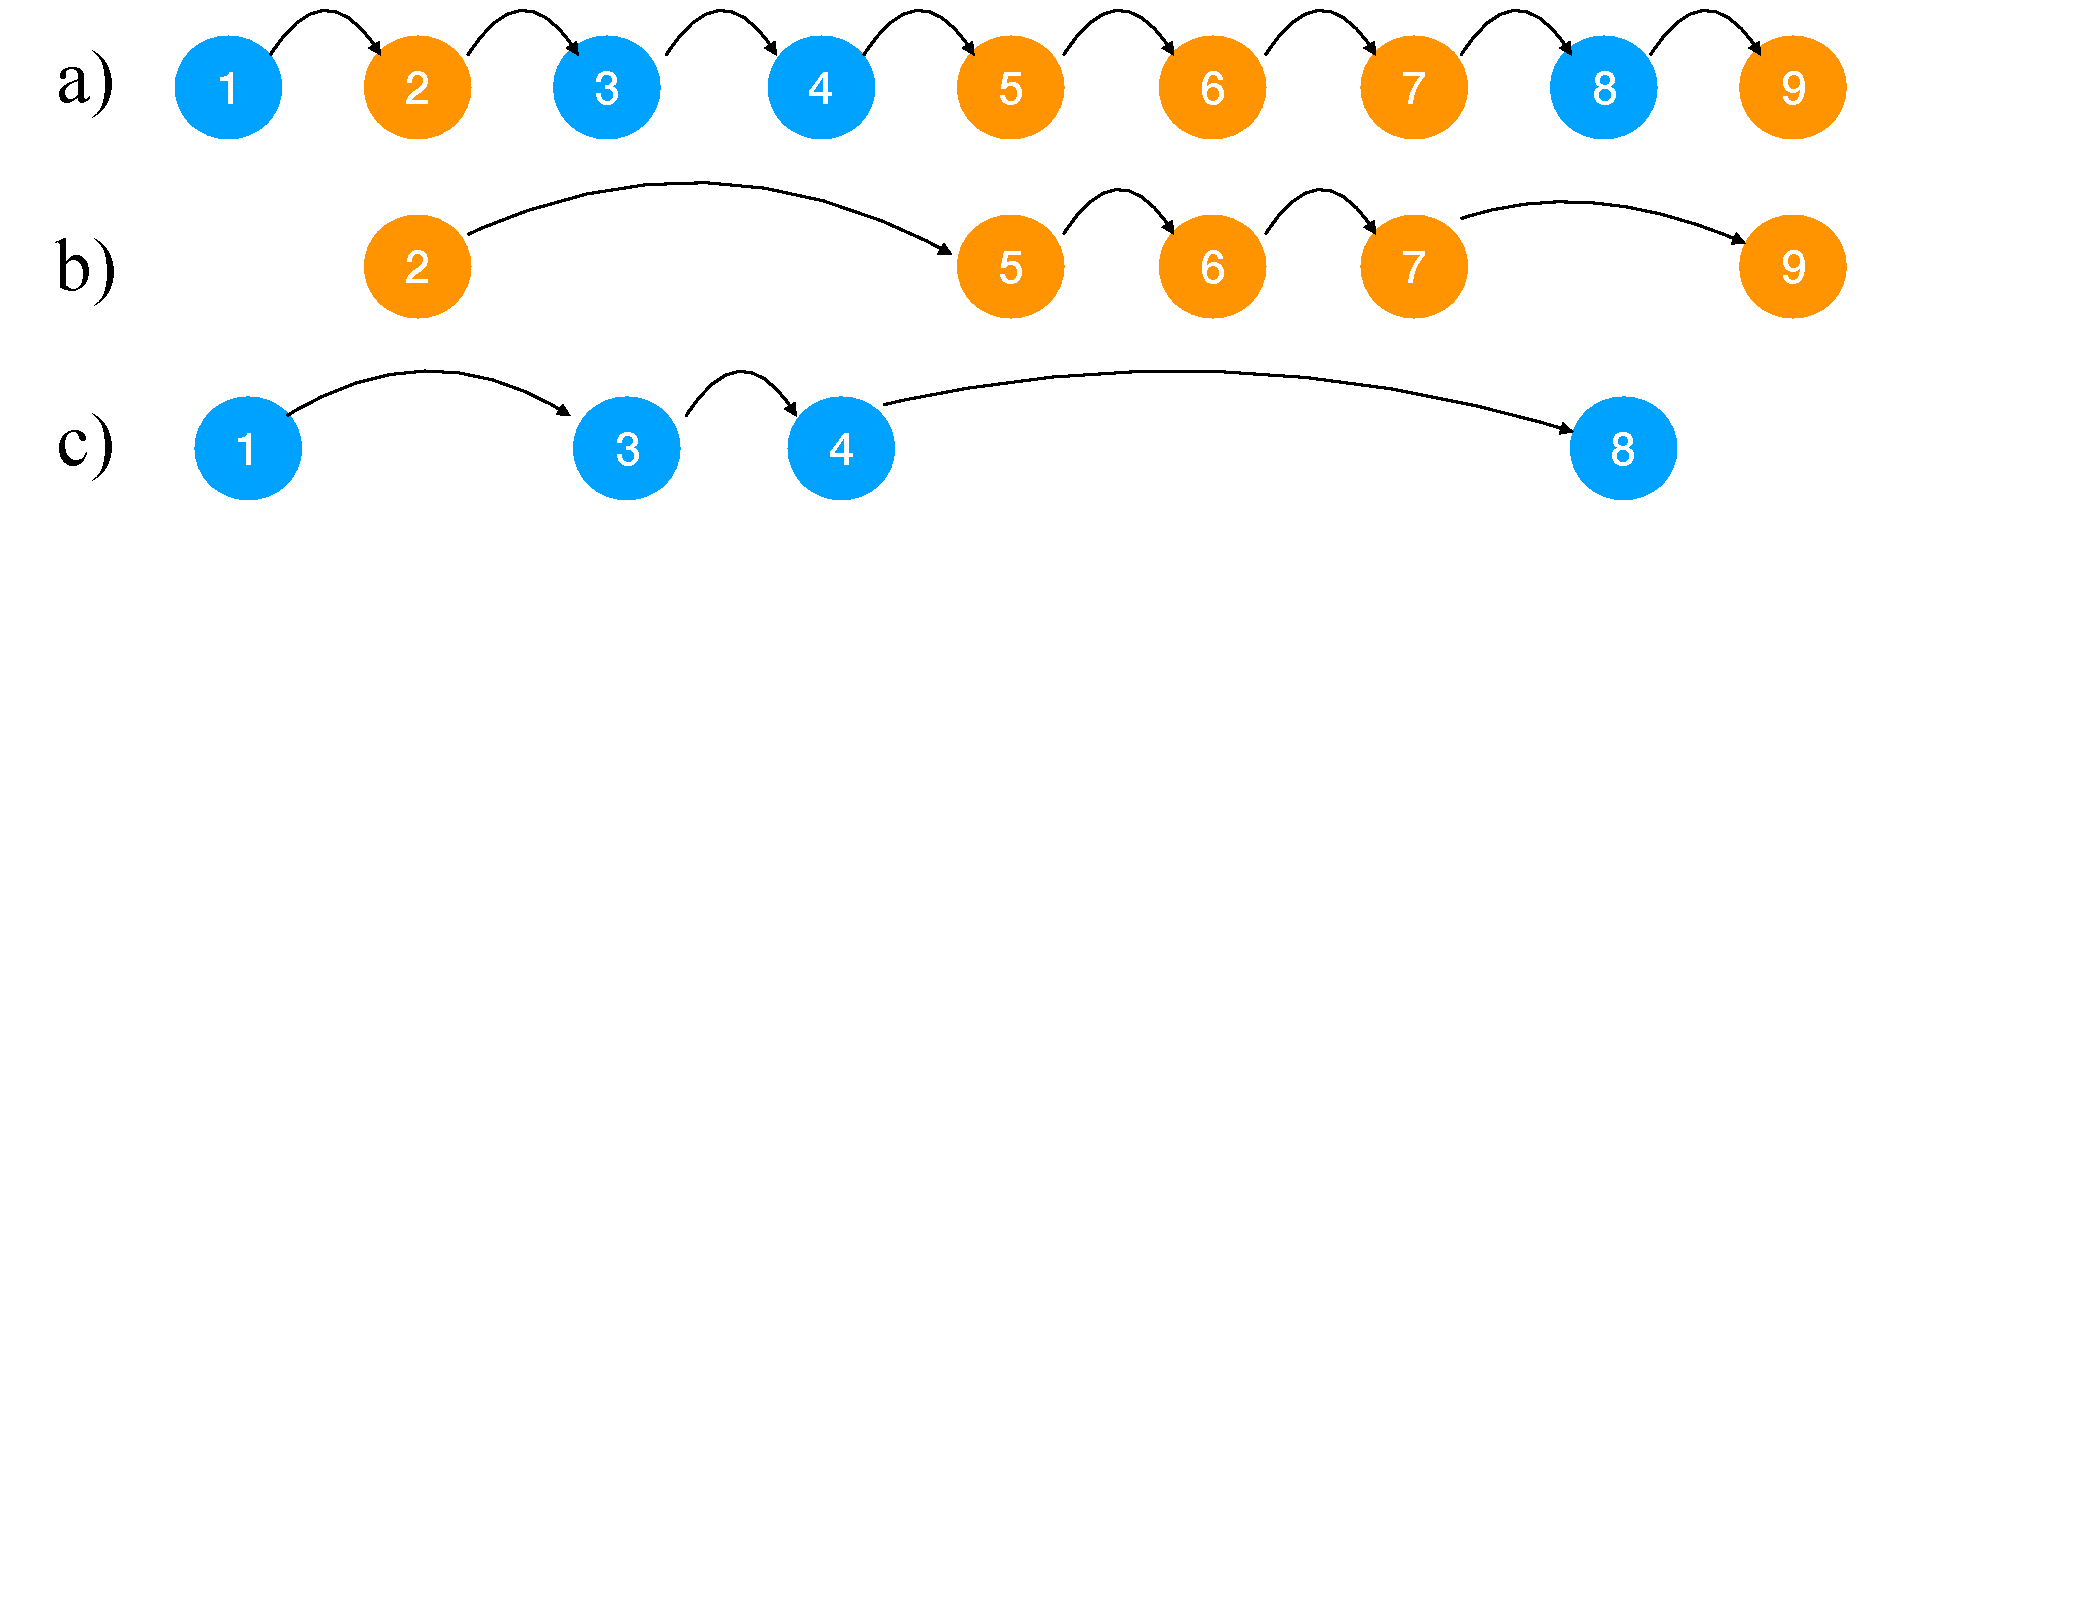
\includegraphics[width=\linewidth]{diagrams/VisibleStates.pdf}
     \end{center}
   \end{minipage}
   \end{center}
   \vspace*{-2.5mm}
   \caption{External States Semantics
     (Def. \ref{def:pair-reduce}). %
     % 
     (a) $\exec{{\color{blue}M} \circ {\color{orange}M'}}{\sigma_1}{\ldots}\leadsto \sigma_9$
     (b) $\reduction{{\color{blue}M}}{{\color{orange}M'}}{\sigma_2}{\ldots}\leadsto \sigma_9$
     (c) $\reduction{{\color{orange}M'}}{{\color{blue}M}}{\sigma_1}{\ldots}\leadsto \sigma_8$
    }
   \label{fig:VisibleStates}
 \end{figure}
 
Fig. \ref{fig:VisibleStates} provides a simple graphical description of 
our external states semantics, showing how given a single execution 
comprised of code from two different modules, we can consider either
the complete execution as in (a), the external state execution when $M_2$ is external (b), and the external state execution when $M_1$ is external  in (c).
 





In this work we are interested in guarantees which are upheld by the internal 
module. Moreover,    these guarantees  need to be satisfied only at `reachable' states,
and need not be satisfied at states that are
not reachable -- this is described formally in Definition \ref{def:arising}. 
Reachable states are those that  may arise by external states execution
of  a given internal module linked with \emph{any} external module.
We describe the states of interest as the \emph{arising states}. 



\begin{definition}[Arising Program State]
\label{def:arising}
For   modules $M_1$ and  $M_2$, a program state $\sigma$ is 
said to be an \emph{arising} state, formally \ \ \ $\arising{M_1}{M_2}{\sigma}$,\ \ \ 
if and only if there exists some $\sigma_0$ such that $\initial{\sigma_0}$ and
$\reductions{M_1}{M_2}{\sigma_0}{\sigma}$.
\end{definition}

% Definition \ref{def:arising} uses the definition for 
In the definition above we used \emph{Initial} states, 
% he definition of which can be found in  Definition \ref{def:initial}. 
\sd{which  characterise states at the start of program execution}.
The heap of an initial state should  contain a single object of class \prg{Object}, and
the  stack should consist of a single frame, whose local variable map contains only the 
mapping of \prg{this} to the single object, and whose continuation may be any statement.
% to be executed.
More in Definition \ref{def:initial}. 
In Definition \ref{def:arising} We also use the notation $\reductions{M_1}{M_2}{\sigma}{\sigma'}$ to denote
zero or more reduction steps starting at state $\sigma$ and ending at state $\sigma$, in the context of internal module 
$M_1$ and external module $M_2$.

Finally, \Loo has a simple class based type system with the following properties:
\begin{description}
\item[(1)]
Classes may be optionally annotated as \prg{enclosed}
\item[(2)]
Methods of non-\prg{enclosed} classes may not return objects of \prg{enclosed} classes
\item[(3)]
Modules are typed in isolation of other modules, thereby implicitly prohibiting
method calls from internal objects to external objects.
\end{description}
The type system is not very important, and fairly simple in it's 
definition. It's only importance is in enforcing the above 
constraints for purposes of encapsulation, a related but somewhat orthogonal 
topic.


\subsection{\SpecO}
\label{sub:SpecO}
\SpecO extends the expressiveness of standard specification languages
with assertion forms capturing key concepts of software security:
 \emph{permission}, \sd{\emph{provenance}}, and \emph{control}.
%That is, \SpecO specifications are able to specify which objects have
%access to which other object (\emph{permission}), whether an object's origin
%is internal or external to known code (\emph{viewpoint}), or which objects call which 
%methods (\emph{control}). 

\subsubsection{Syntax}

\begin{figure}[t]
\footnotesize
\[
\begin{syntax}
\syntaxElement{A}{}
		{
		\syntaxline
				{e}
				{e : C}
				{\neg A}
				{A\ \wedge\ A}
				{A\ \vee\ A}
				{\all{x}{A}}
				{\ex{x}{A}}
		\endsyntaxline
		}
		{
		\syntaxline
				{\access{x}{y}}
				{\internal{x}}
				{\external{x}}
		\endsyntaxline
		}
		{
		\syntaxline
				{\calls{x}{y}{m}{\overline{z}}}
		\endsyntaxline
		}
\endSyntaxElement\\
\end{syntax}
\]
\caption{\SpecO Assertions}
\label{f:chainmail-syntax}
\end{figure}



Fig. \ref{f:chainmail-syntax} gives the assertion syntax of the \SpecO specification language.
An assertion may be an expression, a class assertion, the usual connectives and quantifiers, along 
with the following non-standard assertion forms:
\begin{itemize}
\item
\emph{Permission} ($\access{x}{y}$): % Which objects have access to which other objects (i.e.
  \sd{$x$ has access to $y$}.
\item
{\emph{Provenance}} ($\internal{x}$ and $\external{y}$): %Which objects are internal or external to our component.
 \sd{$x$ is internal, and $y$ is external}.
\item
\emph{Control} ($\calls{x}{y}{m}{\overline{z}}$): 
\sd{$x$ calls method $m$ on object $y$ with arguments $\overline{z}$}.
\end{itemize}
\emph{Permission} and \emph{Provenance} are inspired by the capabilities literature, while
\emph{Control} assists construction of proofs.

\subsubsection{Semantics of \SpecO}
The semantics of \SpecO assertions is given in Definition \ref{def:chainmail-semantics}. 
The definition of the semantics of \SpecO makes use of several language features of 
\Loo that can be found in Appendix \ref{app:loo}. Specifically, $\eval{M}{\sigma}{e}{v}$
is the evaluation relation for expressions, and is interpreted as expression $e$ evaluates
to value $v$ in the context of program state $\sigma$, with module $M$. The full
semantics of expression evaluation are given in Fig. \ref{f:evaluation}. It should 
be noted that expressions in \Loo may be recursively defined, and thus evaluation may not
necessarily terminate, however the logic remains classical because recursion is restricted
to expressions, and not generally to assertions.

Further, Definition \ref{def:chainmail-semantics} uses the interpretation of variables
within a specific frame or state: i.e. $\interpret{\phi}{x} = v$, meaning that $x$ maps to
value $v$ in the local variable map of frame $\phi$, and $\interpret{\sigma}{x} = v$ meaning $x$ 
maps to value $v$ in the top most frame of $\sigma$'s stack. And the term  $\interpret{\sigma}{x.f} = v$
has the obvious meaning.


\begin{definition}[Satisfaction of \SpecO Assertions] 
\label{def:chainmail-semantics}
We define satisfaction of an assertion $A$ by a program state $\sigma$ with internal module $M$ as:
\begin{itemize}
\item
$\satisfiesA{M}{\sigma}{e}$ \ \ \ iff \ \ \  $\eval{M}{\sigma}{e}{\true}$
\item
$\satisfiesA{M}{\sigma}{e : C}$ \ \ \ iff \ \ \  $\eval{M}{\sigma}{e}{\alpha}$ \textit{and} $\class{\sigma}{\alpha} = C$
\item
$\satisfiesA{M}{\sigma}{\neg A}$ \ \ \ iff \ \ \  ${M},{\sigma}\nvDash{A}$
\item
$\satisfiesA{M}{\sigma}{A_1\ \wedge\ A_2}$ \ \ \ iff \ \ \  $\satisfiesA{M}{\sigma}{A_1}$ and 
$\satisfiesA{M}{\sigma}{A_2}$
\item
$\satisfiesA{M}{\sigma}{A_1\ \vee\ A_2}$ \ \ \ iff \ \ \  $\satisfiesA{M}{\sigma}{A_1}$ or 
$\satisfiesA{M}{\sigma}{A_2}$
\item
$\satisfiesA{M}{\sigma}{\all{x}{A}}$ \ \ \ iff \ \ \  
\sd{$\satisfiesA{M}{\sigma[x \mapsto \alpha]}{A}$, \ 
\ \ for some $x$ fresh in $\sigma$, and for all $\alpha\!\in\!\sigma.\prg{heap}$. } 
\item
$\satisfiesA{M}{\sigma}{\ex{x}{A}}$ \ \ \ iff \ \ \  
\sd{$\satisfiesA{M}{\sigma[x \mapsto \alpha]}{A}$, \ 
\ \ for some $x$ fresh in $\sigma$, and for some $ \alpha\!\in\!\sigma.\prg{heap}$. } 
\item
$\satisfiesA{M}{\sigma}{\access{x}{y}}$ \ \ \ iff \ \ \  
\begin{itemize}
\item
$\interpret{\sigma}{x.f}={\interpret{\sigma}{y}}$ \sd{for some $f$}, \  or
\item
there exists some $z$, and some frame $\phi$ in the stack of $\sigma$ such that {$\interpret{\sigma}{x}=\interpret{\phi}{\prg{this}}$}, {and $\interpret{\sigma}{y}=\interpret{\phi}{z}$}
\end{itemize}
\item
$\satisfiesA{M}{\sigma}{\internal{x}}$ \ \ \ iff \ \ \  
$\textit{classOf}(\sigma,x) \in M$
\item
$\satisfiesA{M}{\sigma}{\external{x}}$ \ \ \ iff \ \ \  
$\textit{classOf}(\sigma,x) \not\in M$
\item
$\satisfiesA{M}{\sigma}{\calls{x}{y}{m}{z_1, \ldots, z_n}}$ \ \ \ iff \ \ \ 
\begin{itemize}
\item
$\sigma.\prg{contn} = (\_ := y'.m(z'_1,\ldots,z'_n))$, % and is superfluous, enums are ands, unless expltly stated   
\item
$\satisfiesA{M}{\sigma}{x = \prg{this}}$
%$\interpret{\sigma}{x} = \interpret{\sigma}{\prg{this}}$  % and
\item
$\satisfiesA{M}{\sigma}{y = y'}$
%$\sd{\interpret{\sigma}{y} = \interpret{\sigma}{y'}}$ % and
\item
$\satisfiesA{M}{\sigma}{z_i = z'_i}$\ \ \ for all $1\!\leq i\!\leq n$
%$\interpret{\sigma}{z_i} = \interpret{\sigma}{z'_i}$ \ \ \ for all $1\!\leq i\!\leq n$
\end{itemize}
\end{itemize}
\end{definition}

 
Finally, we define what it means for a module to satisfy an assertion:
a module $M$ satisfies an assertion $A$, if all states $\sigma$
arising from external steps execution of that
module with any other external module, satisfy $A$. 
 
\begin{definition} [Assertion Satisfaction by Modules]
\label{def:mdl-sat}
For a module $M$ and assertion $A$, we say that\ \  $\satisfies{M}{A}$ \ \ if and only if 
for all modules $M'$, and all $\sigma$, if $\arising{M'}{M}{\sigma}$, then $\satisfiesA{M}{\sigma}{A}$.
\end{definition}


% Thus, satisfaction by a module  allows us to talk 
% about what is true for a given module without introducing the 
% details of specific program configurations, a critical component 
% of constructing our Logic of Necessity in Section \ref{s:inference}. 

A proof system for such assertions is indicated by a judgment of the form $\proves{M}{A}$. 
We will not define such a judgment, and just rely on its existence (cf. Theorem 3.2).
We define soundness of such a judgment in the usual way:

\begin{definition}[Soundness of \SpecO Provability]
\label{ax:specW-prove-soundness}
A judgment of the form $M \vdash A$ is \emph{sound}, if for all
  all modules $M$ and assertions $A$, \ if $\proves{M}{A}$ then $\satisfies{M}{A}$.
\end{definition}

\subsubsection{Wrapping}

We define a useful shorthand: the $\wrapped{}$ predicate  states 
that only \internalO objects have access to some object.
That object may be either \internalO or \externalO.
\begin{definition}[Wrapped]
$\wrapped{o}\ \triangleq\ \all{x}{\neg \access{x}{o}\ \vee\ \internal{x}}$
\end{definition}
Wrapped is critical as it captures the conditions under which 
necessitates an interaction
with the \internalM module. If for example, only \internalO
objects have access to an account's password, then
it follows that access to the password may not 
be gained except by an interaction with the \internalM
module, and subsequently if the \internalM module
is secure we know that the password may not be leaked.
 
 

%\begin{figure}[t]
%\begin{mathpar}
%\infer
%		{M;\ M',\ \sigma\ \vdash\ e : \prg{intrnl}}
%		{M;\ M',\ \sigma\ \vdash\ e : \prg{encap}}
%		\and
%\infer
%		{M;\ M',\ \sigma\ \vdash\ e : \prg{intrnl}}
%		{M;\ M',\ \sigma\ \vdash\ e.f : \prg{encap}}
%		\and
%\infer
%		{M;\ M',\ \sigma\ \vdash\ e : \prg{intrnl}}
%		{M;\ M',\ \sigma\ \vdash\ e.g(e') : \prg{encap}}
%\end{mathpar}
%\caption{Encapsulated Expressions}
%\label{f:intrnl}
%\end{figure}
	
%	\begin{figure}[h]
%	\[
%	\begin{array}{llr}
%	A & ::= & \textit{Assertions}\\  
%	| & e & \\
%	| & e\ :\ C & \\
%	| & e\ \in\ S & \\
%	| & A\ \prg{in}\ S & \\
%	| & \access{x}{y} \\
%	| & \internal{x} \\
%	| & \external{x} \\
%%	| & \mut x y f &\\
%%	| & \gives x y z &\\
%	| & \calls{x}{y}{m}{args} \\
%	| & \changes{S}{A} \\
%	| & \neg A & \\
%	| & A\ \wedge\ A & \\
%	| & A\ \vee\ A & \\
%	| & A\ \longrightarrow\ A & \\
%	| & \forall\ x.\ [A] & \\
%	| & \exists\ x.\ [A] & \\
%	| & \forall\ S.\ [A] & \\
%	| & \exists\ S.\ [A] &
%	\end{array}
%%	\begin{array}{llr}
%%	s & ::= & \textit{Source}\\
%%	| & \prg{int} & \\
%%	| & \prg{ext} & \\
%%	| & \_ &
%%	\end{array}
%	\]
%	\caption{Assertions}
%	\label{f:assertions_triple2}
%	\end{figure}





\subsection{\Chainmail -- Necessity Specifications}
\label{s:holistic-guarantees}

\Chainmail extends \SpecO with novel 
\emph{Necessity Specifications}.
In this Section we define the syntax (Fig. \ref{f:holistic-syntax}) and semantics of
\emph{Necessity Specifications}.
We have three forms of Necessity Specifications, defined in Fig. \ref{f:holistic-syntax}, and described below:

\begin{figure}[t]
\footnotesize
\[
\begin{syntax}
\syntaxElement{H}{}
		{
		\syntaxline
				{\onlyIf{A_1}{A_2}{A_3}}
				{\onlyThrough{A_1}{A_2}{A_3}}
%		\endsyntaxline
%		}
%		{
%		\syntaxline
				{\onlyIfSingle{A_1}{A_2}{A_3}}
		\endsyntaxline
		}
\endSyntaxElement\\
\end{syntax}
\]
\caption{Syntax of \Chainmail Necessity Specifications}
\label{f:holistic-syntax}
\end{figure}



\paragraph{Only If}
[$\onlyIf{A_1}{A_2}{A}$]: If an arising program state satisfies $A_1$, and after some execution, a state program state satisfying $A_2$ is reached, 
then the original program state must have also satisfied $A$.
e.g. if the balance of a bank account changes over time, then there must be some external object in the current 
program state that has access to the account's password.

\paragraph{Single-Step Only If}
[$\onlyIfSingle{A_1}{A_2}{A}$]: If an arising program state satisfies $A_1$, and after a single step of execution, a state satisfying $A_2$ is reached, 
then the original program state must have also satisfied $A$.
e.g. if the balance of a bank account changes over a single execution step, then that execution step must be a method call to the bank \prg{transfer} method.

\paragraph{Only Through}
[$\onlyThrough{A_1}{A_2}{A}$]: If an arising program state satisfies $A_1$, and after some execution, a state satisfying $A_2$ is reached, then program execution must have passed through some state satisfying $A$.
e.g. if the balance of an account changes over time, then the bank's \prg{transfer} method must have been called 
in some intermediate state. Note 
that the intermediate state where $A$ is true might be the initial state,
or final state.



All three Necessity Specifications from above talk about assertions satisfied in the 
current state as well as of assertions satisfied in some future state. 
These assertions may contain variables, whose denotation might change during
program execution: the 
map may change, variables may be overwritten, or the entire local variable maps may be lost on a method return.
For this reason, before we provide the semantics of Necessity Specifications, we first introduce an adaptation operator
to account for variable renaming throughout the execution of a program.
\begin{definition}
$\adapt{\sigma'}{\sigma} \triangleq (\chi, \{\prg{local} := \beta[\overline{z} \mapsto \beta(\overline{z}')], \prg{contn}:= [\overline{z'}/\overline{z}]c\} : \psi)$
where 
\begin{itemize}
\item
$\sigma = (\_, \{\prg{local}:=\beta; \prg{contn}:=\_\} : \_)$, and
$\sigma' = (\chi, \{\prg{local}:=\beta', \prg{contn}:=c\} : \psi)$
\item
$dom(\beta') = \overline{z'}$, $dom(\beta) \cap \overline{z} = \emptyset$, and $|\overline{z'}| = |\overline{z}|$
\end{itemize}
\end{definition}

We can now define,  $M \models H$ , the semantics of the Necessity Specifications in Definition \ref{def:necessity-semantics}.  The definition goes by cases over the three possible syntactic forms of $H$: 


\noindent
\begin{definition}[Necessity Specifications]
\label{def:necessity-semantics}
For any assertions $A_1$, $A_2$, and $A$,  we define \\

$\bullet$ \ $\satisfies{M}{\onlyIf {A_1}{A_2}{A}}$ \ \ iff\ \  for all $M'$, $\sigma$, $\sigma'$, such that $\arising{M}{M'}{\sigma}$; \\ % and\\

\begin{tabular}{lr}
$\;\;\;\;$- $\satisfiesA{M}{\sigma}{A_1}$  & \rdelim\}{3}{3mm}[$\;\;\;\Rightarrow\;\;\;$  $\satisfiesA{M}{\sigma}{A}$] \\
$\;\;\;\;$- $\satisfiesA{M}{\sigma' \triangleleft \sigma}{A_2}$   \\
$\;\;\;\;$- $\reductions{M}{M'}{\sigma}{\sigma'}$   \\
\end{tabular}\\ 

$\bullet$ \  $\satisfies{M}{\onlyIfSingle {A_1}{A_2}{A}}$\ \ iff\ \   for all $M'$, $\sigma$,   $\sigma'$, such that $\arising{M}{M'}{\sigma}$: \\

\begin{tabular}{lr}
$\;\;\;\;$- $\satisfiesA{M}{\sigma}{A_1}$  & \rdelim\}{3}{3mm}[$\;\;\;\Rightarrow\;\;\;$  $\satisfiesA{M}{\sigma}{A}$] \\
$\;\;\;\;$- $\satisfiesA{M}{\sigma' \triangleleft \sigma}{A_2}$   \\
$\;\;\;\;$- $\reduction{M}{M'}{\sigma}{\sigma'}$   \\
\end{tabular}\\ 

%% here as it was 
%$\bullet$ \  $\satisfies{M}{\onlyThrough {A_1}{A_2}{A}}$ \ \ iff\ \  for all $M'$, $\sigma$,   $\sigma'$, such that $\arising{M}{M'}{\sigma}$, and \\
%\begin{tabular}{lr}
%$\;\;\;\;$- $\satisfiesA{M}{\sigma}{A_1}$  & 
%\rdelim\}{3}{3mm}%[\makecell{Some really \\ longer text}]
%[$\;\;\;\Rightarrow\;\;\;$\pbox{9cm}{then for all $\sigma_1, \ldots, \sigma_n$ such that $\reduction{M}{M'}{\sigma}{\sigma_1}\leadsto \ldots \sigma_n \leadsto \sigma'$
%there exists some $\sigma_i$ such that $\satisfiesA{M}{\sigma_i \triangleleft \sigma}{A}$ where $0\leq i \leq n$, or $\satisfiesA{M}{\sigma}{A}$, or $\satisfiesA{M}{\sigma' \triangleleft \sigma}{A}$}] \\
%$\;\;\;\;$- $\satisfiesA{M}{\sigma' \triangleleft \sigma}{A_2}$   \\
%$\;\;\;\;$- $\reductions{M}{M'}{\sigma}{\sigma'}$   \\
%\end{tabular}\\ 
%$\bullet$ \  $\satisfies{M}{\onlyThrough {A_1}{A_2}{A}}$ \ \ iff\ \  for all $M'$, $\sigma_1$,   $\sigma_n$, such that $\arising{M}{M'}{\sigma}$: \\
  
$\bullet$ \  $\satisfies{M}{\onlyThrough {A_1}{A_2}{A}}$ \ \ iff\ \  for all $M'$, $\sigma_1$,   $\sigma_n$, such that $\arising{M}{M'}{\sigma_1}$: \\

\begin{tabular}{lr}
$\;\;\;\;$- $\satisfiesA{M}{\sigma_1}{A_1}$  & 
\rdelim\}{3}{3mm}%[\makecell{Some really \\ longer text}]
[$\;\;\;\Rightarrow\;\;\;$\pbox{9cm}{$\forall \sigma_2, \ldots, \sigma_{n-1}$.  \\ 
(\ \ $\forall i\!\in\![1..n).\ \reduction{M}{M'}{\sigma_i}{\sigma_{i+1}}$   \ $\Rightarrow$
$\exists i\!\in\![1..n]. \  \satisfiesA{M}{\sigma_i \triangleleft \sigma_1}{A}$ \ \ )   }] \\
$\;\;\;\;$- $\satisfiesA{M}{\sigma_n\triangleleft \sigma}{A_2}$   \\
$\;\;\;\;$- $\reductions{M}{M'}{\sigma}{\sigma_n}$   \\
\end{tabular} 
\end{definition} 



 
With the necessity specifications as defined in Definition \ref{def:necessity-semantics},
we are able to state what are the necessary preconditions to critical functions in 
software, including safety properties of software in the open world. The semantics
of \emph{Single-Step Only If} allow for the statement of such necessary preconditions
for any execution step for any program to achieve a certain outcome. The semantics
of \emph{Only If} and \emph{Only Through} allow us to raise these necessary preconditions
to any arbitrary number of execution steps, and thus allow for reasoning about 
the execution of an entire program.
 
Looking back at the example from the Introduction,   it holds that
\\
\strut $\hspace{1in}$ \prg{Mod1} $\models$ \prg{NecessityBankSpec}
 \\
\strut $\hspace{1in}$ \prg{Mod2} $\not\models$ \prg{NecessityBankSpec}
 \\
\strut $\hspace{1in}$ \prg{Mod3} $\models$ \prg{NecessityBankSpec}
 

 
As further examples of Necessity Specifications, consider the original 
bank account example discussed in Section \ref{s:intro}. We have already shown
how we can specify knowledge of an account's password using \prg{NecessityBankSpec},
but we are also able to write other useful properties about the bank account. 
 
\begin{lstlisting}[language = Chainmail, mathescape=true, frame=lines]
NecessityBankSpec'  $\triangleq$  from a:Account $\wedge$ a.balance==bal
                       to1 a.balance < bal
                       onlyIf $\exists$ o.[$\external{\texttt{o}}$ $\wedge$ $\calls{\prg{o}}{\prg{a}}{\prg{transfer}}{\prg{\_, \_, \_}}$]
\end{lstlisting}
 
\prg{NecessityBankSpec$^\prime$} states that if over a single step the balance of an account decreases, then it must have occurred as 
a result of a call to \prg{transfer}.
 
\begin{lstlisting}[language = Chainmail, mathescape=true, frame=lines]
NecessityBankSpec''  $\triangleq$  from a:Account $\wedge$ a.password == pwd
                        to a.password != pwd
                        onlyThrough $\exists$ o.[$\external{\texttt{o}}$ $\wedge$ $\calls{\prg{o}}{\prg{a}}{\prg{set}}{\prg{pwd, \_}}$]
\end{lstlisting}
 
\prg{NecessityBankSpec$^{\prime\prime}$} states that if over an arbitrary number of execution steps, the password of an account changes,
then it follows that there must have been some intervening execution step that was a call to \prg{set} on the account 
with the correct password. Both of these specifications are important, and are both used as intermediate steps
when we present the full proof of \prg{NecessityBankSpec} later in Section \ref{s:examples}.

Necessity Specifications thus provide us with a rich language for talking about the necessary conditions
under which critical actions within of our software are allowed to occur. 
\jm[]{It is worth discussing the semantics of necessity specifications and their 
relation to typical logical consequence and Hoare logic. A classical Hoare triple, 
$\hoare{P}{C}{Q}$, denotes that any program state that satisfies $P$, after execution 
of program $C$, will result in a program state that satisfies $Q$. Thus, $P$ represents 
a subset of program states that after execution of $C$ results in a program state satisfying $Q$.
Conversely, $Q$ represents a superset of program states resulting from the execution of $C$ in 
a program state satisfying $P$. Thus, we can soundly strengthen the left hand side ($P$), and weaken
the right hand side ($Q$). This intuition extends to all three necessity specifications. 
For example, from \prg{NecessityBankSpec'}, while it is somewhat contrived, we are able to
strengthen the ``left hand side'' by adding information, and weaken the ``right hand side'', 
and conclude that}
\begin{lstlisting}[language = Chainmail, mathescape=true, frame=lines]
NecessityBankSpec'''  $\triangleq$  from a:Account $\wedge$ a.balance == bal $\wedge$ bal == x + y $\wedge$ y > 0
                       to1 a.balance == x
                       onlyIf $\exists$ o.[$\external{\texttt{o}}$ $\wedge$ $\access{\prg{o}}{\prg{a}}$]
\end{lstlisting}
\jm[]{This follows because in the above specification, (a)\prg{x < bal}, and thus \prg{a.balance = x} implies and $a.balance < bal$,
and (b) if an object calls a method on another object, it follows that it has access to that object.
More generally, given an Single-Step Only-If necessity specification, 
$\onlyIfSingle{A_1}{A_2}{A}$, $A_1$ and $A_2$ represent a subset of single step execution paths starting from a program state 
satisfying $A_1$ and reaching a program state satisfying $A_2$, that have $A$ as a necessary precondition. 
In the same way the converse is true, i.e. $A$ represents a superset of initial program states
for execution starting at a state satisfying $A_1$ and reaching a state satisfying $A_2$ after a single step of execution.
As with Hoare logic, we are able to soundly strengthen the left hand side ($A_1$ and $A_2$)
and strengthen the right hand side ($A$). This intuition also extends to Only-If and Only-Through necessity specifications. 
In some places later in this paper, we use the distinction ``\emph{left hand side}'' of a necessity specification
to denote the two left most assertions in the specification, and ``\emph{right hand side}'' to denote
the necessity precondition.}
 




\subsection{Encapsulation}
\jm[lemmas? does A => enc(A') imply A => enc($\neg$A')?]{}
 %In order to reason about necessary requirements in an open world,
% and those assertions that may change due 
% to computation by external, unknown code.
\sd{In the introduction we used the concept of encapsulation of \SpecO assertions 
 when proving adherence to \Chainmail Necessity Specifications.}
An assertion $A$ is encapsulated by a module $M$ if it cannot be invalidated unless an
internal method is called. 
\sd{Here we refine this concept, to allow for ``conditional'' encapsulation:
$M\ \vDash A\ \Rightarrow\ \encaps{A'}$ expresses that in states which satisfy $A$, the assertion 
$A'$ cannot be invalidated, unless a method from $M$ was called.}

\begin{definition}[Assertion Encapsulation]
\label{def:encapsulation}
For % an internal module. -- SDL internal is nit an inherrent property
a module $M$ and assertion $A$, we define an assertion $A'$ as being 
encapsulated, written\ \  $M\ \vDash A\ \Rightarrow\ \encaps{A'}$, \ \ if and only if
%$M\ \vDash\ \onlyIfSingle{A}{\neg A}{\calls{x}{y}{m}{\overline{z}}\ \wedge\ \external{x}\ \wedge\ \internal{y}}$
for all external modules $M'$, and program states $\sigma$ and $\sigma'$
such that $\arising{M}{M'}{\sigma}$:

\begin{tabular}{lr}
$\;\;\;\;$- $\reduction{M}{M'}{\sigma}{\sigma'}$  & \rdelim\}{4}{3mm}[$\;\;\;\Rightarrow\;\;\;$  $\exists x,\ \overline{z}. (\satisfiesA{M}{\sigma}{\calls{\_}{x}{m}{\overline{\sd{z}}}\ \wedge\ \internal{x}})$] \\
$\;\;\;\;$- $\satisfiesA{M}{\sigma}{A}$   \\
$\;\;\;\;$- $\satisfiesA{M}{\sigma}{A'}$   \\
$\;\;\;\;$- $\satisfiesA{M}{\sigma' \triangleleft \sigma}{\neg A'}$   \\
\end{tabular}
\end{definition}
